\documentclass[a4paper, 12pt]{article}
\usepackage[margin=0.8in]{geometry}
\usepackage{tikz}
\usepackage{scrextend}
\usetikzlibrary{automata,positioning}
\usepackage{graphicx}
\usepackage{pgfplots}
\usepackage{listings}
\usepackage{color}

\definecolor{comments}{rgb}{0,0.5,0.5}
\definecolor{typeWord}{rgb}{0.5,0,1}
\definecolor{number}{rgb}{1,0.5,0}
\definecolor{string}{rgb}{0.5,0.5,0.5}

\lstset{frame=tb,
  language=Java,
  aboveskip=3mm,
  belowskip=3mm,
  showstringspaces=false,
  columns=flexible,
  basicstyle={\small\ttfamily},
  numbers=none,
  numberstyle=\color{number},
  commentstyle=\color{comments},
  stringstyle=\color{string},
  keywordstyle=\color{typeWord},
  breaklines=true,
  breakatwhitespace=true,
  tabsize=4
}

\title{Scotland Yard AI}
\author{Julian Loscombe and Ben Milne}

\begin{document}
\maketitle
\section{Game Tree}
We have set up our game tree to use Alpha - Beta pruning in order to increase the depth that we can search to in the allotted time. In addition we are allowing our tree to generate throughout the game, pruning off branches of unreachable nodes as moves are made.
\subsection{Iterative Depth Search}
Because we have a strict time limit in order to make our move and given that the initial conditions change the complexity of the game tree, we have decided to use an iterative depth search, updating the best move on each iteration and simply grabbing the one that is available when the time limit is near.
\subsection{Scoring}
To score our game state we use three main sources of information, the ratio between the PageRank of the detectives' locations and Mr X's location, the ratio between the value of the detectives and MrX's tickets, and the average distance between the detectives and Mr X (using Dijkstra's Algorithm). We consider the average distance to be the most important factor and as such its influence is weighted much higher than the other two. Because it is particularly important to avoid very small distances we use a root function to transform the distance score so that is is much steeper when Mr X is close to being caught. We then normalise the ratios around 0 and apply them to the distance score as below:
\begin{lstlisting}
double score = (10 * Math.pow(detDistance, 0.5));
        score += ((ticketRatio - 1) * kTicketInfluence) * score;
        score += ((pageRankRatio - 1) * kPageRankInfluence) * score;
\end{lstlisting}
This ensures that the average ratio will have no effect on the score and that when the distance is very small it's main objective is to increase that distance. We also added a special case to boost secret move scores when the distance was very small. The below graph illustrates part of the score function.

\begin{figure}[!h]
\centering
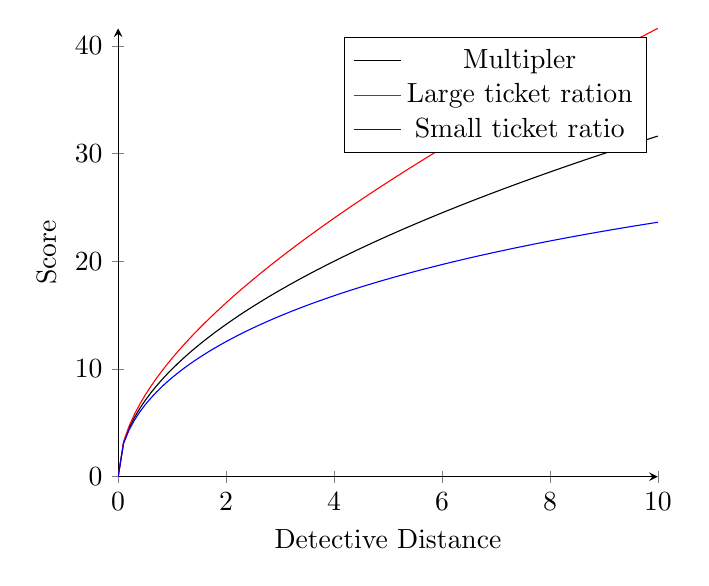
\begin{tikzpicture}
\begin{axis}[
    axis lines = left,
    xlabel = {Detective Distance},
    ylabel = {Score},
]
%Below the red parabola is defined
\addplot [
    domain=0:10, 
    samples=100, 
    color=black,
]
{(1-1)*x + (1-1)*x + 10*x^0.5};
\addlegendentry{Multipler}
%Below the red parabola is defined
\addplot [
    domain=0:10, 
    samples=100, 
    color=red,
]
{(2-1)*x + (1-1)*x + 10*x^0.5};
\addlegendentry{Large ticket ration}
%Here the blue parabloa is defined
\addplot [
    domain=0:10, 
    samples=100, 
    color=blue,
    ]
    {(0.2-1)*x + (1-1)*x + 10*x^0.5};
\addlegendentry{Small ticket ratio}
 
\end{axis}
\end{tikzpicture}
\end{figure}
\subsection{Pruning}
We are hoping to keep the tree running throughout the game in order to use the work we have already done to extend the depth we are able to reach. Clearly though, we must prune branches that are made impossible by the game advancing in order to make any real progress. We achieve this by setting the root of the tree to be the node containing the last played move, thus making unneeded nodes unreachable. However, what if we are currently in one of those pruned branches? We would waste time evaluating nodes that are unnecessary. So, to avoid this, we perform a quick when we enter our alphabeta() function to see if we have pruned and break out if this is the case
\begin{figure}[h!]
  \centering
  	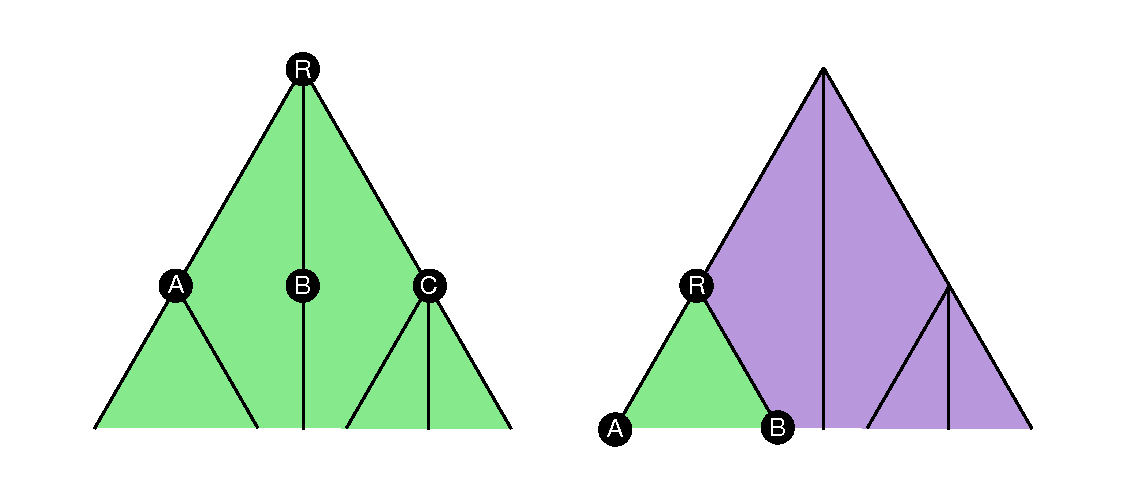
\includegraphics[width = 17cm]{TreePruning}\\
  \caption{After making move A, we can prune all other moves and their subsequent moves.}
\end{figure}
\section{Results}
The AI we have produced has very promising results and does make smart moves. However, we are still coming up against erro
\end{document}










